\section{Тестове}
\begin{Large}
	Тестовете са изпълнени на машина със следната конфигурация: CPU - AMD Ryzen 1700 3.0GHz, 8 ядра, 16 нишки, общо кеш L1-768KB, L2-4MB
,L3-16MB; RAM - DDR4 16GB ок.3000MHz.
\begin{enumerate}
\item Grayscale оцветяване с гранулярност 1
\newline
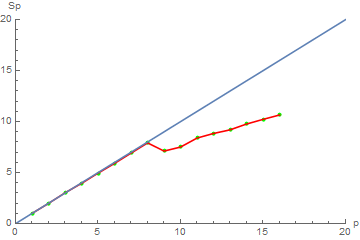
\includegraphics[scale=1]{tt1}

\item Grayscale оцветяване с гранулярност 5
\newline
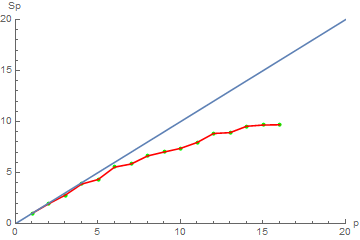
\includegraphics[scale=1]{tt2}
\item Просто многоцветно оцветяване с гранулярност 1
\newline
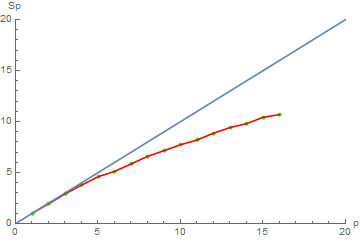
\includegraphics[scale=1]{tt3}
\item Просто многоцветно оцветяване с гранулярност 5
\newline
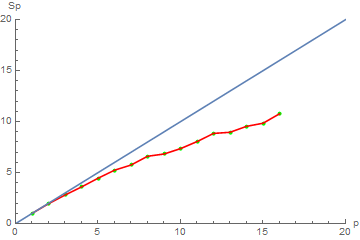
\includegraphics[scale=1]{tt4}
\end{enumerate}
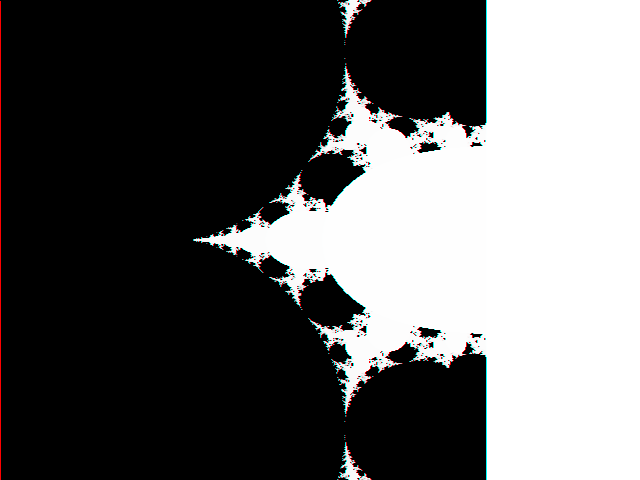
\includegraphics[scale=1]{test1.16}
\newline
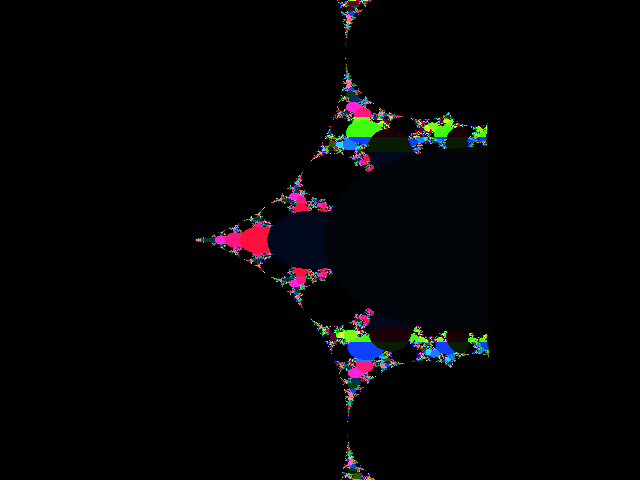
\includegraphics[scale=0.8]{test3.1}
\end{Large}